% Drawing 144/09-2 -- folder 144, batch 09, archive page 163 (PDF page 164).
% Transcription: à gauche, un tore dessiné en perspective, avec deux cercles méridiens et des courbes en pointillés ; à droite, un carré de sommets $a_0, a_1, a_2, a_3$ (côté $a_0a_1$ fléché), un petit carré intérieur, deux axes fléchés $e'$ (horizontal) et $e''$ (vertical), avec les légendes $\tau' = \mathrm{id}$ et $\tau'' = \ill{}$.
% Kind: torus in perspective; square a_0..a_3 with axes e', e''. Method 2 (schematic redraw from the facsimile). Status: ok.
% Notes: Left: torus with two meridian circles and dashed curves. Right: the square a_0 a_1 a_2 a_3 (side a_0a_1 arrowed), a small inner square, the axes e' (pointing left, as drawn) and e'' (up), legends tau' = id and, under the vertical axis, tau'' = ... Disagreement (notes only): the transcription leaves the tau'' legend illegible; on the facsimile it looks like "tau'' = c^te", as on p. 159. The label epsilon(X) above the square is text and not drawn.
% Coordinates: 1 unit = 1 mm = 1/100 of the crop width (bbox in page fractions: [0.08, 0.58, 0.6, 0.75]).
% Redrawn by Claude (claude-opus-5-5), issue #73, 2026-11-07; not checked by a human; not compiled (no TeX in the session).
% Rights: reproduces part of the work -- behind RENDER_TRANSCRIPTS, never published by itself.
\documentclass[tikz,border=3pt]{standalone}
\usepackage{amsmath,amssymb}
\usetikzlibrary{patterns,arrows.meta}
\tikzset{pencil/.style={black!45}, struck/.style={black!35}, mark/.style={circle,draw,inner sep=1.3pt}, pt/.style={circle,fill,inner sep=0.9pt}, opt/.style={circle,draw,fill=white,inner sep=1.1pt}}
\begin{document}
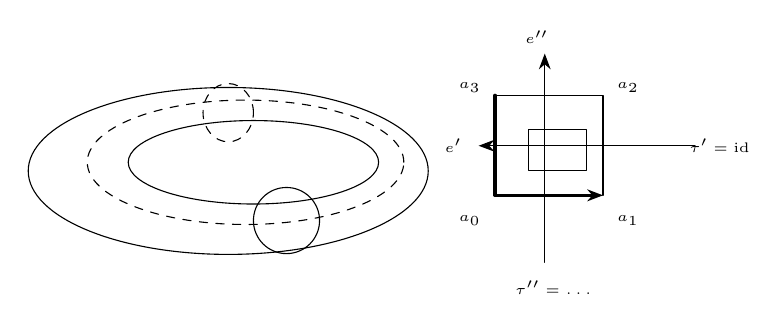
\begin{tikzpicture}[x=1mm,y=1mm,line cap=round,line join=round,font=\scriptsize]
\draw (36.5,-28.6) ellipse[x radius=25.4, y radius=10.6];
\draw (39.7,-27.5) ellipse[x radius=15.9, y radius=5.3];
\draw[dashed] (38.7,-27.5) ellipse[x radius=20.1, y radius=7.9];
\draw[dashed] (36.5,-21.2) ellipse[x radius=3.2, y radius=3.7];
\draw (43.9,-34.9) ellipse[x radius=4.2, y radius=4.2];
\draw (70.4,-19) -- (84.1,-19) -- (84.1,-31.7);
\draw[very thick,{Stealth[length=2mm]}-] (84.1,-31.7) -- (70.4,-31.7);
\draw[very thick] (70.4,-31.7) -- (70.4,-19);
\draw (74.6,-23.3) -- (82,-23.3) -- (82,-28.6) -- (74.6,-28.6) -- cycle;
\draw[-{Stealth[length=2mm]}] (95.8,-25.4) -- (68.3,-25.4);
\draw[-{Stealth[length=2mm]}] (76.7,-40.2) -- (76.7,-13.7);
\node[inner sep=1pt] at (65.1,-25.4) {\tiny $e'$};
\node[inner sep=1pt] at (75.7,-11.6) {\tiny $e''$};
\node[inner sep=1pt] at (98.9,-25.4) {\tiny $\tau'=\mathrm{id}$};
\node[inner sep=1pt] at (77.8,-43.4) {\tiny $\tau''=\ldots$};
\node[inner sep=1pt] at (67.2,-18) {\tiny $a_3$};
\node[inner sep=1pt] at (87.3,-18) {\tiny $a_2$};
\node[inner sep=1pt] at (67.2,-34.9) {\tiny $a_0$};
\node[inner sep=1pt] at (87.3,-34.9) {\tiny $a_1$};
\end{tikzpicture}
\end{document}
